\section{Modeling}
This section details common prediction methods and then highlights our novel methodology that captures matchup specific factors. As a means for motivation, consider claims of the type ``\emph{team i is a tough matchup for team j due to their ...}'' often made by sports broadcasters. There are two ways to consider this statement: (i) the overall team strength of team $i$ will be problematic for team $j$ or (ii) team $i$ has certain tendencies above and beyond their team strength that will pose difficulties for team $j$. We outline a general framework for the first case, specifying models that account for differences in team strength. However, for the second case a different approach is needed to analytically quantify characteristics that pose difficulties for a given team. Many traditional methods, particularly those based on rankings, impose a characteristic we deem transitivity on predictions. While transitivity is fully in coming sections, the key point is that models with this property rely on estimates of team strength and are unable to adapt and computer specific tendencies of a given matchup. Hence, we introduce the Nearest-Neighbor Matchup Effect which captures characteristics of specific match ups and doesn't adhere to transitivity in predictions.  

\subsection{Data Treatment}
For our purposes game summary data is used, but another approach not explored here focuses on simulating each sequence in a game as in \cite{vstrumbelj2012} rather than the final outcome. There are a few necessary data considerations when modeling game outcomes, specifically whether the outcome of a game is binary (win/loss) or continuous (point differential) as well as whether linear or non-linear modeling (in the predictors) should be used. For the first dilemma involving whether the outcome should be modeled in a binary or continuous sense, point spread provides a means for eliciting the relative strength of one team. Although as any basketball fan can attest to the final score is often not indicative of how the closeness of the game. Nevertheless, point spreads are informative about the relative strength of one team compared to another. In practice, given a posterior distribution of point spreads, the transformation to win probability is straightforward.  In regards to the second consideration, our experience showed that non-linear methods such as CART provided little extra predictive power when compared to linear methods. This is particularly the case when using a selection of rating systems.

\subsection{Relative Strength Models}
Adopting the continuous treatment of game outcomes (e.g. point spread) we next detail models designed to capture the relative strength of two teams. The general form for the relative strength models is:
\begin{eqnarray}
Y_{ijk} = g_1(X_{ij}) + g_2(X_i) + g_3(X_j) +  \epsilon_{ijk}
\label{eq:RS}
\end{eqnarray}
where $Y_{ijk}$ is the point differential between teams $i$ and $j$ for matchup $k$.  The covariate matrix $X_{ij} = \{x_{ij1}, ..., x_{ijp_1}\}$ corresponds to the difference in covariates for teams $i$ and $j$, where for instance $x_{ij1} =$ Sagarin rating team $i$ - Sagarin rating team $j.$  The covariate matrix $X_l = \{x_{l1}, ..., x_{lp_2}\}$ contains predictors for team $l$, and $\epsilon_{ijk} \sim N(0,\sigma^2)$ is the error for the $kth$ matchup between teams $i$ and $j$. A simple example,but surprisingly useful example of Equation~\ref{eq:RS} would be a simple linear model:
\begin{eqnarray}
Y_{ijk} = X_{ij}\beta + \epsilon_{ijk}.
\label{eq:RS_Linear}
\end{eqnarray}
\subsection{Calibrating Probabilities}
Given a posterior predictive distribution for point spread between teams $i$ and $j$, $Y_{ijk},$ it is a straightforward transformation to recover win probability. Consider Figure \ref{fig:winprob} which displays the distribution of point differential and corresponding win probability for a team favored to win by 5 points (e.g. $E[Y_{ijk}]=5$).
\begin{figure}[h!]
\centering
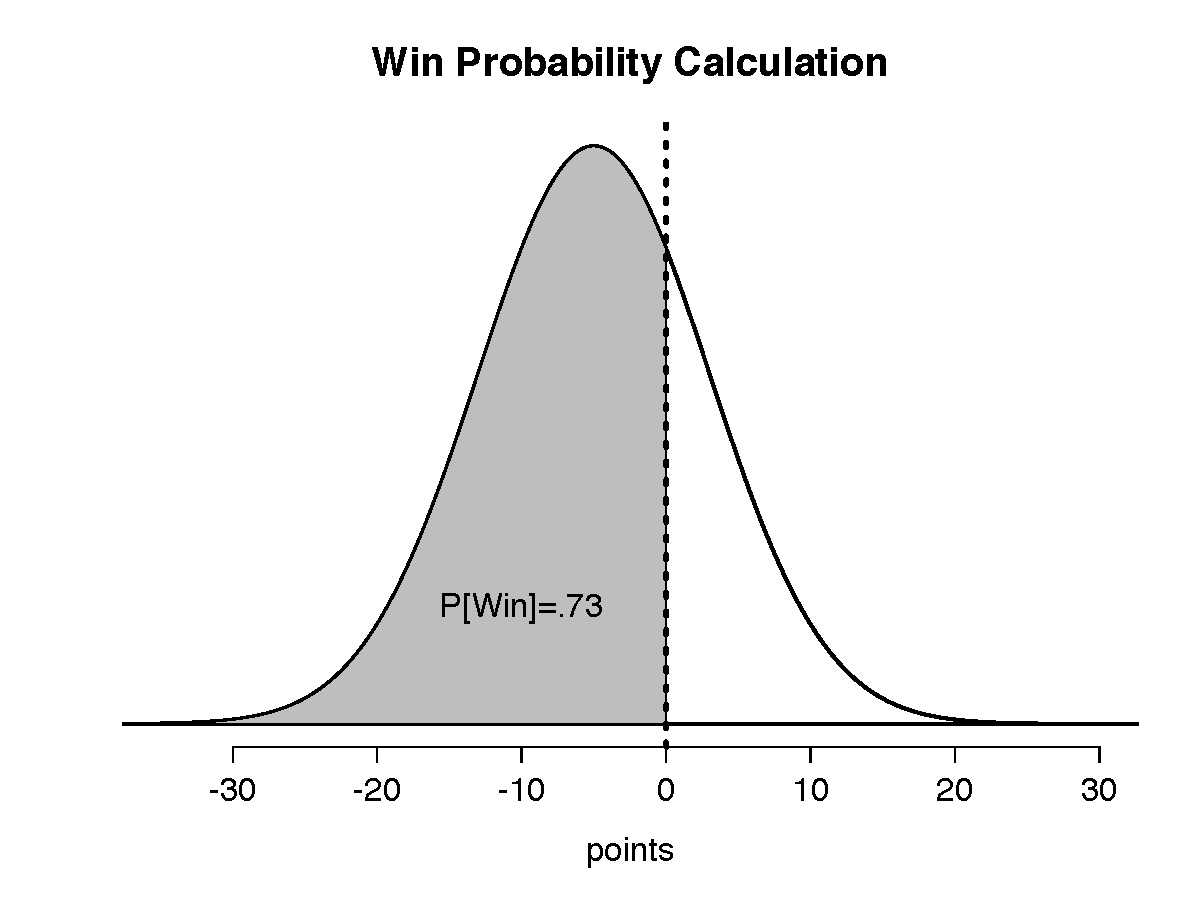
\includegraphics[width=.9\textwidth]{WinProb.pdf}
\caption{Calculating win probability from point differential}
\label{fig:winprob}
\end{figure} 
While the actual variance of the posterior predictive distribution will vary, the distribution displayed in Figure \ref{fig:winprob} is $Normal(5,11^2).$

\subsection{Popular Methods}  This section provides a review of several existing methods for tournament prediction.
\subsubsection{Rating Based Methods} 
The seeds and ratings discussed earlier contain implicit or explicit means for tournament prediction. For instance the Sagarin rankings are designed to reflect the point spread between two teams, incorporating a term for the variance of the outcomes under a Bayesian framework provides an efficient way to compute win probabilities. Similarly for any of the other rankings coefficients for predicting point spreads or in a binary regression can be computed. A seed based probability is shown in \cite{schwertman1996}. A more sophisticated approach using point spreads along with Sagarin rankings is shown in \cite{carlin1996}. A method that allows team strength to vary in shown in \cite{glickman1998}.
\subsubsection{Ensemble Methods}
Combining the ratings from several different sites is a popular strategy. In fact this is the technique used by Nate Silver's 538 methodology. In particular Nate Silver's model incorporates 7 sets of rankings: Sagarin's, Pomeroy's, LRMC, Sonny Moore power ratings, ESPN's Basketball Power Index (BPI), NCAA selection committee ``S-curve'', and Associated Press preseason poll along with injuries and distance required to travel to construct power ratings (\cite{silver}). Similar to Sagarin's ratings, the rating difference between two teams are designed to reflect an estimated point spread. In general model averaging proved useful, smoothing out over fitting or model biases.  \cite{silver} goes on to say:
\begin{quote}
One of the ways I was able to look smart over the past six years, during which time I spent a lot of effort on political forecasting, was by betting on the favorite. I wasn't literally placing bets, mind you (unless you want to count my proposed bet with Joe Scarborough). But for some reason, in political prognostication, you can be regarded as a savant just by pointing out that the favorite is probably going to win.

The standard in sports prediction is higher. And this year's NCAA basketball tournament is designed to make me look dumb. There aren't any favorites. Sure, some teams are better bets than others. (I wouldn't advise staking your fortune on Cal Poly.) But the team that our statistical model regards as the favorite to win it all, Louisville (more on the Cardinals in a moment), has just a 15 percent chance of doing so. In other words, there�s an 85 percent chance that Louisville won't cut down the nets again and that I'll be wrong.
\end{quote}
\andyc{Consider sliding this up to intro along with Pomeroy quote}
\subsection{Nearest-Neighbor Matchup Effects}
The nearest-neighbor matchup effects are tailored for the second scenario in which there exist team level characteristics - above and beyond team strength - that contribute to win probability. For instance, maybe a certain team struggles with taller teams that rebound well. When facing an opponent with these attributes the team would expect to perform worse than the difference in team strengths would suggest. This is plausible as the team strength is calculated across a variety of opponents, hence we search for a subclass of opponents in which the strengths differ from the overall mean. Our procedure is a three step process: (i) fit a relative strength model of the form specified in Equation~\ref{eq:RS}, (ii) identify neighbors, by finding similarities between the current opponent and past opponents for each team, and (iii) calibrate the matchup adjustment. Fitting of the relative strength model follows the same form as previously described and will not be rehashed in this segment. Our example model which is fully detailed in the following following section follows the form of Equation \ref{eq:RS_Linear} using the Sagarin ratings as predictors.
\subsubsection{Choosing Neighbors}
When choosing neighbors for a matchup between team $i$ and team $j$, we need to identify past opponents of team $i$ with similar attributes to team $j$ and past opponents of team $j$ with similar attributes to team $i.$ The idea is to identify how the performance changes against that subset of opponents relative to the overall relative strength computed on the entire set of opponents a team as faced.

There are a multitude of ways to select the neighbors. In particular one needs to consider what variables to include for selecting neighbors, how should those variables be weighted if at all, and how many neighbors should be selected. We consider a large set of team level data from which a 5-nearest neighbor approach is calculated. In particular we use over twenty variables equally weighted for the nearest neighbor calculation including: team height, adjust tempo, percentage of scoring from 3 pointers, offensive rebound percentage, free throw percentage, block percentage, steal rate, and many others.

Typically this procedure would be done analytically, however, user input can also be solicited. For instance, suppose that a user decided Mercer was similar to Wake Forest and Clemson. In this case current and ongoing work in Bayesian Visual Analytics (BAVA) framework detailed in \cite{house2010}  and \cite{hu2013} provides a principled routine for visualizing teams and taking user input of similarities to create a method for computing distance between teams. Specifically this is a way to weight clustering variables to reflect user preferences.
\subsubsection{Matchup Adjustment}
The idea of the matchup adjustment is to quantify how much a team underperformed (or over performed) relative the expected team strength for a subset of teams similar to the current opponent. For instance, if team $i$ was two points better than expected against teams similar to $j$, then it would be reasonable to assume that team $i$ would perform better against team $j$ as well.  Assume a simple linear model from Equation \ref{eq:RS_Linear}, then the predictive distribution for a matchup between team $i$ and team $j$ now becomes 
\begin{eqnarray}
p(Y_{ij}|X_{ij}, \beta,\sigma^2,\mathcal{N}_i^k(j),\mathcal{N}_j^k(i), \rho) &\sim& N(\epsilon_{ij}, \sigma^2) \label{eq:ME}
\\
\epsilon_{ij} &=& X_{ij} \beta + \rho(\mathcal{N}_i^k(j) -\mathcal{N}_j^k(i)),
\end{eqnarray}
where $\mathcal{N}_j^k(i)$ is the average residual for the team $i's$ $k$ past opponents most similar to team $j$ and $\rho$ is a tuning parameter $\in [0,1]$ that controls the amount of information passed from similar neighbors. The same idea applies to more general model specified in Equation \ref{eq:RS}.

\subsubsection{Calibrating the Matchup Adjustment}
The natural support of $\rho$ would be between zero and one.  The interpretation of the extreme points is rather intuitive - with $\rho = 0$ Equation~\ref{eq:ME} reverts to Equation~\ref{eq:RS} and with $\rho = 1$ the entire residual for similar teams is retained. To select $\rho$ in practice, we recommend a historical analysis to calibrate $\rho$ for the current year's predictions. For the relative strength model and nearest neighbor variables used in this work, $\rho$ near 0.2 performed optimally across the historical data.   \andyc{maybe add the plot Marcos suggested here}.

\subsection{A note about Transitivity}
The transitive property states if $A>B$ and $B>C$ then $A>C$. In terms of basketball prediction consider:
\begin{eqnarray}
P_{A,B} > 0.5 \quad \& \quad P_{B,C} > 0.5 \rightarrow P_{A,C} > 0.5,
\label{eq:trans}
\end{eqnarray}
where $P_{I,J}$ is the probability of team I defeating team J.  We deem Equation \ref{eq:trans} a transitive property for basketball prediction. That is if team A is expected to beat team B and team B is expected to beat team C, then team A should also defeat team C. Note these are probabilities not true outcomes, due to the parity in basketball inferior teams can and often do defeat stronger teams. Any sort of relative strength model would require this transitive ordering holds, home court effects non-withstanding. On the other hand, our matchup effects modeling approach can determine if the strengths of a given team present difficulties for a specific team meaning the transitive property is not required to hold and $P_{A,B} > 0.5 \quad \& \quad P_{B,C} > 0.5\quad \& \quad P_{A,C} < 0.5$ is valid.
